
%(BEGIN_QUESTION)
% Copyright 2010, Tony R. Kuphaldt, released under the Creative Commons Attribution License (v 1.0)
% This means you may do almost anything with this work of mine, so long as you give me proper credit

Examine this P\&ID and answer the following questions:

$$\includegraphics[width=15.5cm]{i04742x01.eps}$$

\vskip 10pt

Identify the ``normal'' mode of operation for this system as specified by the process engineer who built it: the status of the process (ball) valve and of both solenoid valves during typical process operations when all is well.

\begin{itemize}
\item{} Solenoid valve \#1: {\it pass-thru} or {\it vent}?
\vskip 10pt
\item{} Solenoid valve \#2: {\it pass-thru} or {\it vent}?
\vskip 10pt
\item{} Process valve: {\it open} or {\it shut}?
\end{itemize}

\underbar{file i04742}
%(END_QUESTION)





%(BEGIN_ANSWER)

\begin{itemize}
\item{} (3 points) Solenoid valve \#1: {\bf vent}
\vskip 10pt
\item{} (3 points) Solenoid valve \#2: {\bf vent}
\vskip 10pt
\item{} (4 points) Process valve: {\bf open}
\end{itemize}


%(END_ANSWER)





%(BEGIN_NOTES)

{\bf This question is intended for exams only and not worksheets!}

%(END_NOTES)


